\documentclass[a4paper, 10pt, twocolumn]{scrartcl}
\usepackage[ngerman]{babel}

% Mathematics
\usepackage{amsmath}
\usepackage{amssymb}
\numberwithin{equation}{subsection}
\numberwithin{figure}{section}
\numberwithin{table}{section}

% Font and Style
\usepackage{ucs}
\usepackage[T1]{fontenc}
\usepackage{abstract}
\usepackage{url}
\usepackage{lipsum}
\usepackage{hyperref}
\hypersetup{colorlinks=false}

% Source Code Highlighting
\usepackage{caption}
\usepackage[section]{minted}
\usemintedstyle{trac}
\setminted[java]{autogobble,mathescape,fontfamily=courier,breaklines,fontsize=\footnotesize}
\renewcommand{\listingscaption}{Quellcode}

% Font Package (select one)
%\usepackage{lmodern}
%\usepackage{kpfonts}
%\usepackage{ccfonts}
%\usepackage[light]{cmbright}
%\usepackage{antpolt}
\usepackage[]{iwona}

% Bibliography
\usepackage[numbers,round]{natbib}
\usepackage[babel,german=guillemets]{csquotes}
\bibliographystyle{alphadin}

% Image and Graphics
\usepackage{graphicx}
\usepackage{dblfloatfix}
\usepackage[left=2.3cm, right=2.3cm, top=2.5cm, bottom=4.5cm]{geometry}
\setlength{\columnsep}{15pt}
\setlength{\columnseprule}{0.0pt}

% Document Information
\title{Robby Projekt}
\subtitle{Erweiterung des Greenfoot Roboter-Szenarios um Sensorik, Speicher und  Hindernisumgehung}
\author{Adrian Schrader \and Moritz Jung \and Alexander Riecke}
\date{\today}

\begin{document}
  % Create Title, Abstract and TOC
  \twocolumn[\maketitle \begin{abstract} \begin{minipage}{1.0\linewidth}
  \lipsum[1]

  \vspace{0.8cm}
  \end{minipage}\end{abstract} ]

  \tableofcontents

  % CONTENT
  \section{Implementierung}
  \section{Sensorik}

\subsection{Aufgabenstellung}
Um Robby Anhaltspunkt für seine Aktionen zu geben, sollen zwei verschiedene Arten von Sensoren eingeführt werden, mit denen Robby seine Umgebung abtasten kann. Robby kann nicht durch eine Wand laufen, also sollte er erkennen können, ob in seiner Umgebung solch ein Hindernis auftaucht.

Eines der Hauptaktionen eines Roboters in diesem Szenario ist das Sammeln von Akkus für Energie. Um gezielter nach Akkus suchen muss Robby seine Umgebung nach ihnen abtasten.

\paragraph{wandHinten()}
Wenn, in Bezug auf Robbys Laufrichtung gesehen, ein Actor der Klasse Wand ein Feld hinter Robby steht, soll die Methode \mintinline{java}{true} zurückgeben, ansonsten \mintinline{java}{false}.

\paragraph{akkuVorne() [ akkuRechts(), akkuLinks() ]}
Wenn, in Bezug auf Robbys Laufrichtung gesehen, ein Actor der Klasse Akku ein Feld vor [rechts von, links von] Robby steht, soll die Methode true zurückgeben, ansonsten false.

\subsection{Problematik}

\subsection{Lösung}

  \section{Speicher}

\subsection{Aufgabenstellung}
\lipsum[2]

\subsection{Problematik}
\lipsum[3]

\subsection{Lösung}
\lipsum[4-5]

  \subsection{Hindernisse}

\subsubsection*{Aufgabenstellung}
Aufgabenstellung war es, Robby ein geschlossenes Hindernis aus Wänden umrunden zu lassen, so dass er nach erfolgreicher Umrundung wieder am Ausgangspunkt ankommt.
Auch die Weltgrenze wird als Hindernis wahrgenommen

\subsubsection*{Problematik}
Als augenscheinlich einfachste Lösung stellte sich eine Verkettung von mehreren if-Abfragen heraus, in der nacheinander von Rechts beginnend gegen den Uhrzeigersinn die einzelnen möglichen vewegungsrichtungen abgefragt wurden. Diese Lösung erwies sich jedoch als sehr verschachtelt, da für jede Abfrage eine einzelne Reaktionsanweisung erstellt werden musste.
Weiterhin konnten anfangs nur sehr begrenzte Tests durchgeführt werden, da die Funktion in einem Ablauf ausgeführt wird und somit keine Möglichkeit besteht, auch weitergehende Aufgaben währenddessen auszuführen.


\subsubsection*{Lösung}
Durch Einführen einer do-while-Schleife und einer for-Schleife für die Abfragen der Umgebung, also der Wände und Weltgrenzen auf benachbarten Feldern, konnte der Code auf ein Minimum reduziert werden, in dem  zwar immernoch von Rechts beginnend die Umgebung angefragt wird, jedoch die Funktion immer wieder mit anderen Winkel aufgerufen wird und nicht für jede Richtung eine neue Abfrage geschrieben werden muss.
Auch eine Möglichkeit zum Ausführen von weiterem Code während der Umrundung wurde Implementiert, um beispielsweise auch weitergehende Aufgaben, wie zum Beispiel das Ablegen von Schrauben zu ermöglichen, aber auch , um zu die zu Testzwecken benötigten Daten während der Umrundung zu erfassen.


  \section{Funktionstests}
  Zum Überprüfen der Funktionalität haben wir eine Testengine entworfen. Die Klasse \emph{FeatureTest} bietet mit der Funktion \mintinline{java}{boolean testAllFeatures()} die Funktionalität aller beschriebenen Funktionalitäten zu überprüfen.

Um eine automatische Funktionsüberprüfung nach dem kompilieren zu erreichen, wurde die Klasse \mintinline{java}{RoboterWelt} erweitert, damit Sie den Test starten kann. Im Prinzip des OOP wurden jedoch alle Tests in einer seperaten Klasse durchgeführt.

Die Klasse \mintinline{java}{FeatureTest} bietet das Grundgerüst für die Testengine. Hier sind die Methoden zu Hause, die reflexiv auf Robby zugreifen, um die Rückgabewerte seiner Methoden zu überprüfen oder Felder auszulesen.

In der \mintinline{java}{FeatureTest} erweiternden Klasse \mintinline{java}{RobbyTest} sind die unten beschriebenen Testabläufe implementiert. Die volle Umsetzung aller im Lastenheft angeforderten Funktionen ist gelungen und wird zu Beginn jedes Programms mit einem Testlog, der bspw. in Abbildung~\ref{img:testlog} zu sehen ist, bestätigt.

\begin{figure}
\centering
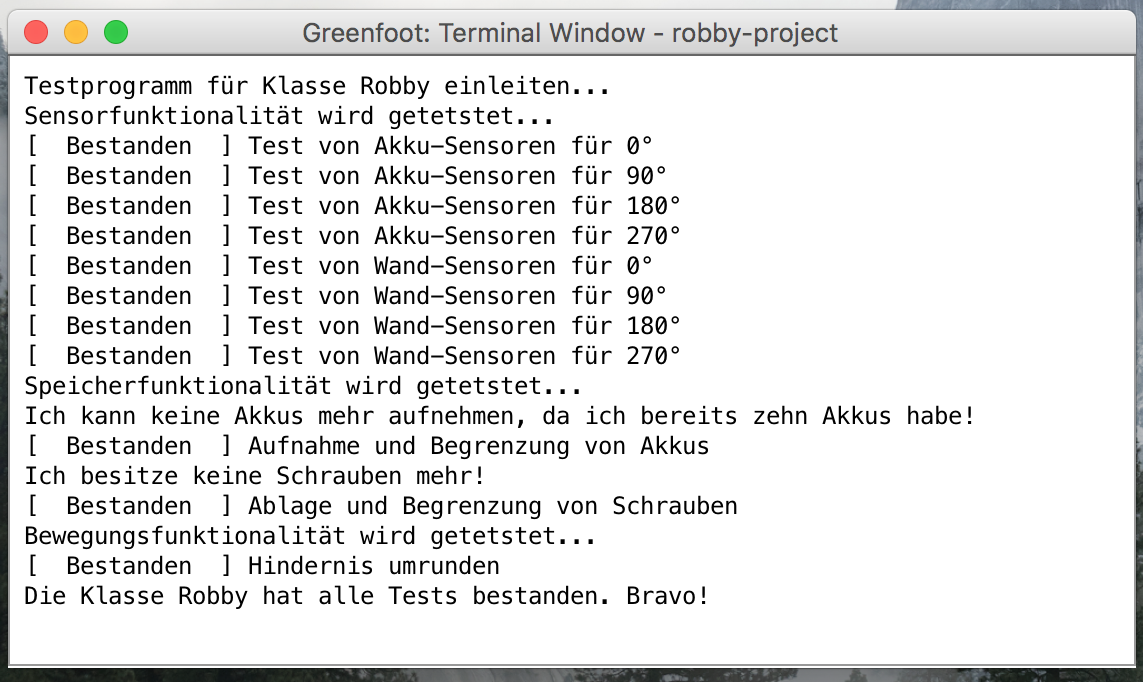
\includegraphics[width=\linewidth]{img/testlog}
\caption{Erfolgreicher Testlog nach dem Kompilieren der Klassen. }
\label{img:testlog}
\end{figure}

\subsection{Sensorik}
Robbys Sensorfunktionen für Akkus und Wände, die im Rahmen dieses Projekts erweitert wurden, sollen die jeweiligen Spielfiguren positiv, sowie negativ nachweisen können. Falsch positive und falsch negative Ergenisse müssen ausgeschlossen werden. Jede Funktion muss au\ss{}erdem in unterschiedlichen Blickrichtungen getestet werden, um Zufallstreffer auszuschlie\ss{}en.

Im Gegensatz zur Implementierung der Funktionen in Robby müssen die Testfunktionen wasserdicht sein. Deduktive mathematische Beweise werden daher durch das ausprobieren jedes möglichen Falls in jeder Ausgangssituation getestet.

\subsubsection*{Testablauf}
Robby wird in Schleifen durch die verschiedenen Situationen/Winkel iteriert. Es wird für jeden Blickwinkel ($0^\circ, 90^\circ, 180^\circ$ und $270^\circ$) überprüft, ob die zuständige Funktion erkennt, dass kein Objekt neben Robby liegt und dass sich nach dem Einfügen des gesuchten Objekts neben Robby der Test positiv ausfällt. Die Objekte werden danach wieder aufgeräumt und aus der Welt entfernt.

\subsubsection*{Situationen: }
Drehungen um $0^\circ, 90^\circ, 180^\circ$ und $270^\circ$

  \subsection{Speicher}
Die Test sollen überprüfen, ob Robby beim Einsammeln oder Ablegen von Objekten auch sein Inventar im Speicher aktualisiert.

\subsubsection*{Testablauf}
\textbf{Akkus} Robby wird immer wieder auf einen Akku gestellt und die Funktion zum einsammeln ausgeführt. Nach jedem Durchgang wird geprüft, ob Robby den Speicher um eins hochgezählt hat, die Variablengrenzen zwischen 0 und 10 nicht überschritten wurden und das Objekt tatsächlich entfernt wurde. Siehe \mintinline{java}{boolean testObjectAquisition(String, String, int, Class<?>)} in Quellcode \ref{lst:robbytest}.

\textbf{Schraube} Die Funktion zum Ablegen wird wiederhohlt ausgeführt. Nach jedem Durchgang wird geprüft, ob Robby den Speicher um eins runtergezählt hat, die Variablengrenze von 0 nicht unterschritten wurden und das Objekt tatsächlich hinzugefügt wurde. Siehe \mintinline{java}{boolean testObjectDeposition(String, String, int, Class<?>)} in Quellcode \ref{lst:robbytest}.

  \subsection{Hindernisse und Bewegung}
Die Test sollen überprüfen, ob Robby ein geschlossenes Hindernis aus Wänden umrunden kann ohne Kontakt zur Wand zu verliehren und wieder am Ausgangspunkt ankommt.

\subsubsection*{Testablauf}
Robby wird in der Welt mit Blickrichtung zur Wand platziert und um ihn herum ein Hindernis, wie in Abbildung~\ref{img:obstacle} dargestellt, aufgabaut. Da die Implementierung von \mintinline{java}{void hindernisUmrunden(Runnable)} ermöglicht, Benutzeraktionen während des Umrundens durchzuführen, wird getestet, ob sich in den acht Feldern um Robby eine Wand befindet. Wenn nicht ist der Test gescheitert. Auch muss gewährleistet sein, dass er am Ende wieder an der Ausgangsposition ankommt und die Spielfläche aufgeräumt wird.

\begin{figure}
\centering
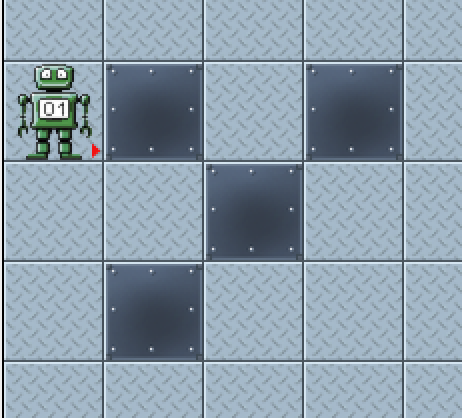
\includegraphics[width=0.8\linewidth]{img/obstacle}
\caption{Das von der Testfunktion erstellte Hindernis. }
\label{img:obstacle}
\end{figure}


  \section{Gruppenarbeit}
Aus den Funktionsanforderungen des Lastenhefts für die Klasse Robby und die Dokumentation haben wir kleinere Aufgabenpakete zusammengestellt, die in der Gruppe verteilt werden können.

\begin{table*}
    \centering
    \caption{Aufgabenübersicht und Zuständigkeiten des Projekts}
    \begin{tabular}{ l l l }
        \textbf{Bereich} & \textbf{Aufgabe} & \textbf{Zuständigkeit}\\ \hline\hline
        Sensorik & Funktionalität implementieren & Adrian \\
                 & Sourcecode kommentieren & Adrian \\
                 & Sourcecode aufräumen, anpassen und zusammenfügen & Adrian \\
                 & Schriftliche Dokumentation & Adrian \\ \hline
        Speicher & Funktionalität implementieren & Alex \\
                 & Sourcecode kommentieren & Alex \\
                 & Sourcecode aufräumen, anpassen und zusammenfügen & Adrian \\
                 & Schriftliche Dokumentation & Alex \\ \hline
       Hindernis & Funktionalität implementieren & Moritz \\
                 & Sourcecode kommentieren & Moritz \\
                 & Sourcecode aufräumen, anpassen und zusammenfügen & Adrian / Moritz \\
                 & Schriftliche Dokumentation & Moritz \\ \hline
        Tests    & Planung & Adrian \\
                 & Funktionalität implementieren & Adrian \\
                 & Sourcecode kommentieren & Adrian \\
                 & Sourcecode aufräumen, anpassen und zusammenfügen & Adrian \\
                 & Schriftliche Dokumentation & Adrian \\ \hline
    \end{tabular}
\end{table*}

\subsection*{Sourcecode-Verwaltung}
Um den Überblick über den aktuellen Stand zu behalten und die Sourcecodeversionen koordinert zusammenführen zu können, haben wir gehostete git-Repositorys mit Issuetrackern und Milestones eingerichtet. Nach Abgabe der Dokumentation sind diese auch öffentlich verfügbar. Das Robbyprojekt ist unter \url{https://github.com/adrianschrader/robby-project} und die Dokumentation als \LaTeX-Projekt unter \url{https://github.com/adrianschrader/robby-project-doc} zu finden.


  \onecolumn{
    \section{Anhang: Vollständiger Quellcode}
    Alle geänderten oder hnzugefügten Klassen werden im Folgenden aufgeführt. Die Zeilenangaben links entsprechen denen im Greenfoot-Szenario.

    \subsection{Robby.java}
    \label{lst:robby}
    \inputminted[firstline=1,linenos,numbers=left]{java}{code/Robby.java}

    \subsection{FeatureTest.java}
    \label{lst:featuretest}
    \inputminted[firstline=1,linenos,numbers=left]{java}{code/FeatureTest.java}

    \subsection{RobbyTest.java}
    \label{lst:robbytest}
    \inputminted[firstline=1,linenos,numbers=left]{java}{code/RobbyTest.java}

    \subsection{RoboterWelt.java}
    \label{lst:roboterwelt}
    \inputminted[firstline=1,linenos,numbers=left]{java}{code/RoboterWelt.java}

  }


\end{document}
